\documentclass[a4wide]{report}

\usepackage{amsmath}
\usepackage[a4paper, total={7in, 10.2in}]{geometry}
\usepackage{graphicx}
\usepackage[portuguese]{babel}
\usepackage[utf8]{inputenc}


\begin{document}

\noindent
{\bf Rafael V. Cacilhas  - Relatório 14 (\today)}

\vspace{0.5cm}

\section*{Exercício 1}

\subsection*{a) }
Na Figura \ref{1a} está representado o número de prisioneiros que escolhem cooperar em função do tempo para 4, 8 e 16 vizinhos respectivamente. Note que há uma rápida convergência para o valor de equilíbrio, sendo necessárias apenas 2 iterações em alguns casos. 
\begin{figure}[!htb]
\centering
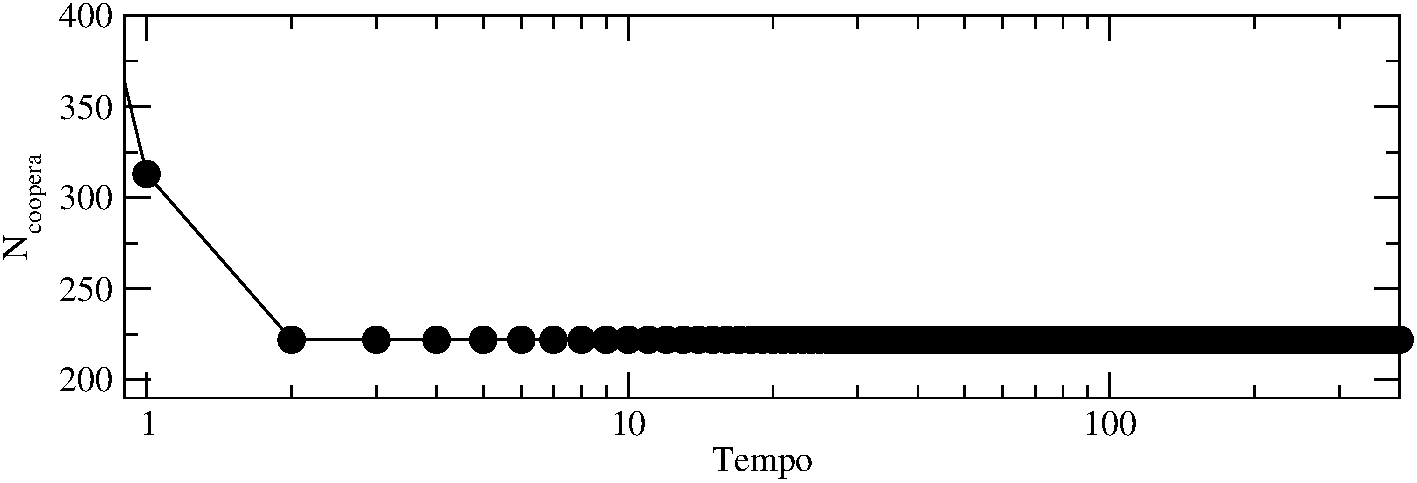
\includegraphics[width=0.4\textwidth]{az4.pdf} \newline
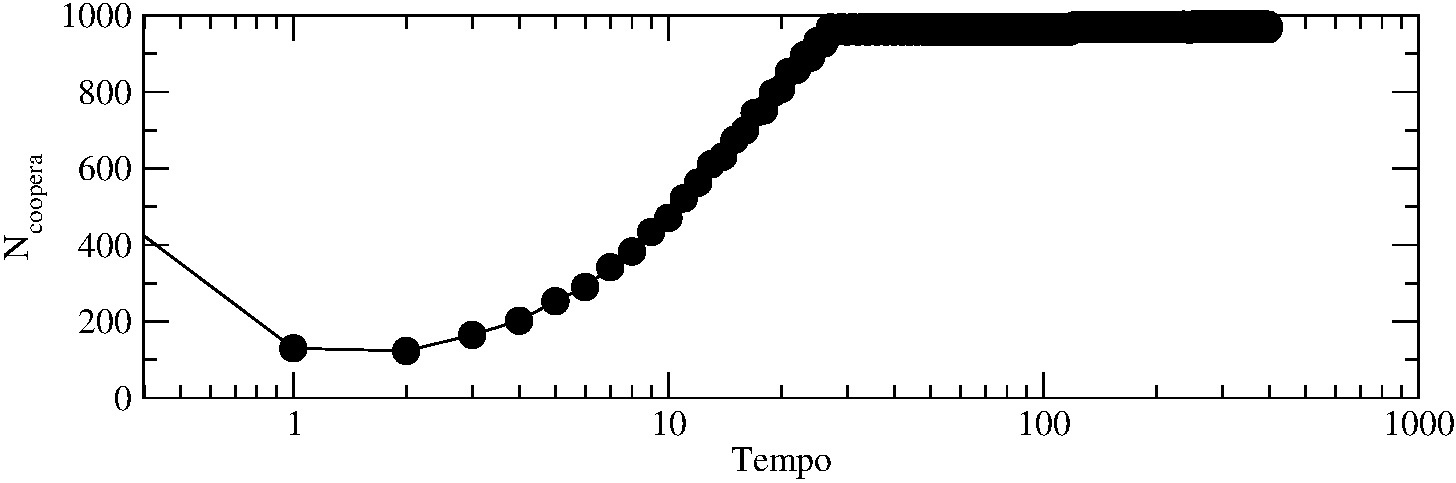
\includegraphics[width=0.4\textwidth]{az8.pdf} \newline
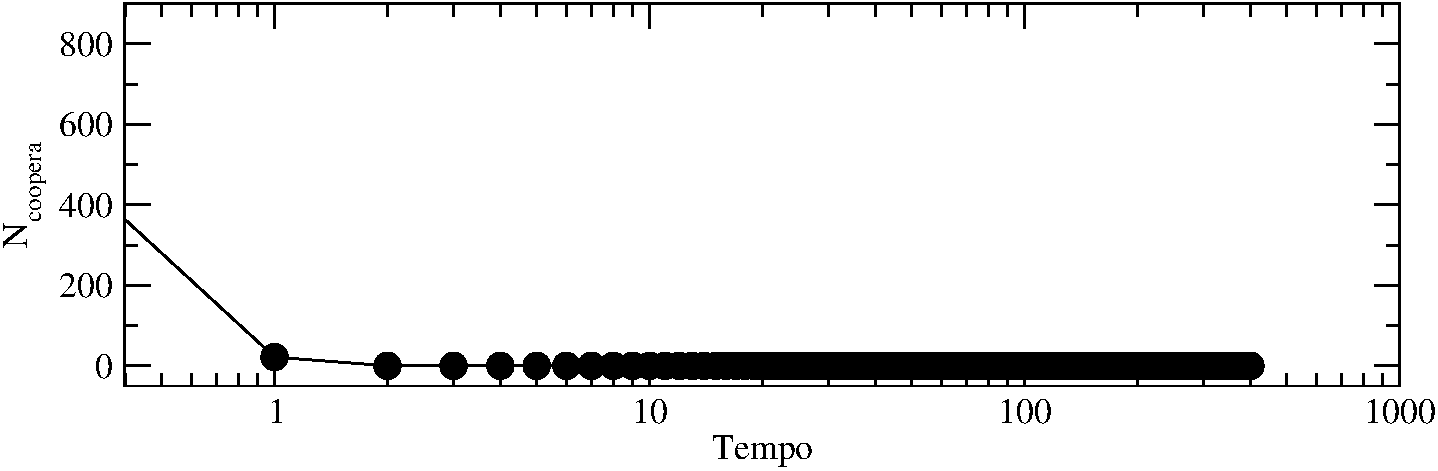
\includegraphics[width=0.4\textwidth]{az16.pdf}\newline
\caption{Número de prisioneiros cooperando em função do tempo para 4, 8 e 16 vizinhos respectivamente.}
\label{1a}
\end{figure}

É interessante notar também como a mudança do número de vizinhos z faz com que o comportamento mude bruscamente de uma convergência em $N \approx 225$ (z = 4), $N \approx 1000$ (z = 8) e $N \approx 0$ (z = 16).


\subsection*{b) }
Nas Figuras \ref{1b} - \ref{3b} à seguir foi marcado de preto ao longo do eixo x a posição espacial de cada prisioneiro cooperador e o eixo y representa a passagem de tempo. Como visto acima, o caso z = 8 possui uma alta densidade de indíviduos cooperadores, então foi escolhido plotar para este caso os indivíduos delatores para facilitar a visualização. 

\begin{figure}[!htb]
\centering
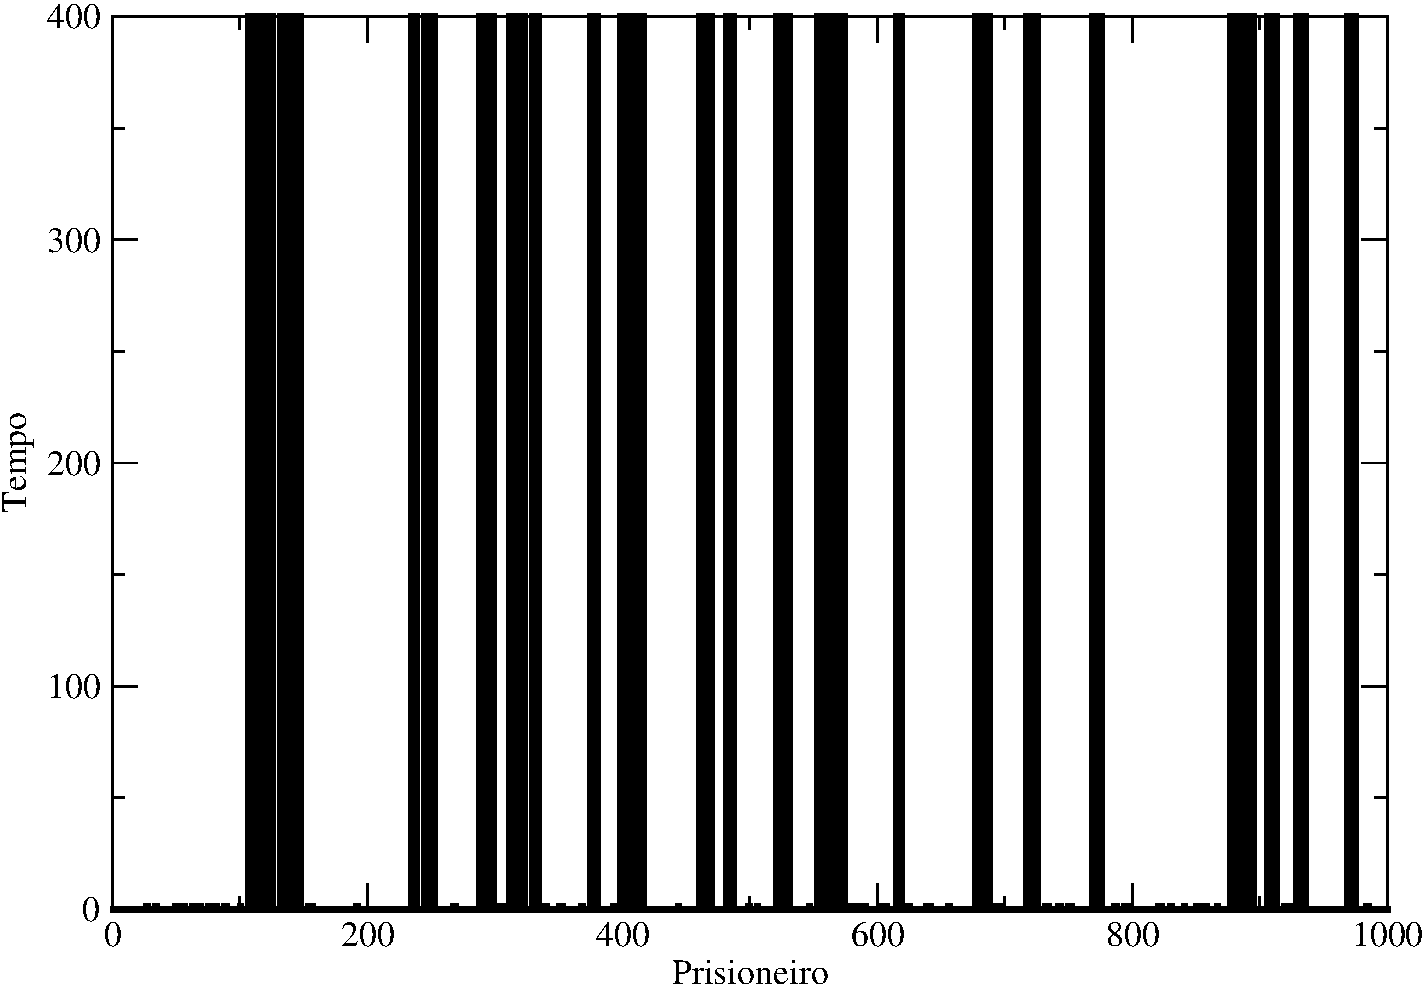
\includegraphics[width=0.4\textwidth]{z4.pdf}
\caption{Posição dos prisioneiros cooperando em função do tempo para z = 4.}
\label{1b}
\end{figure}

\begin{figure}[!htb]
\centering
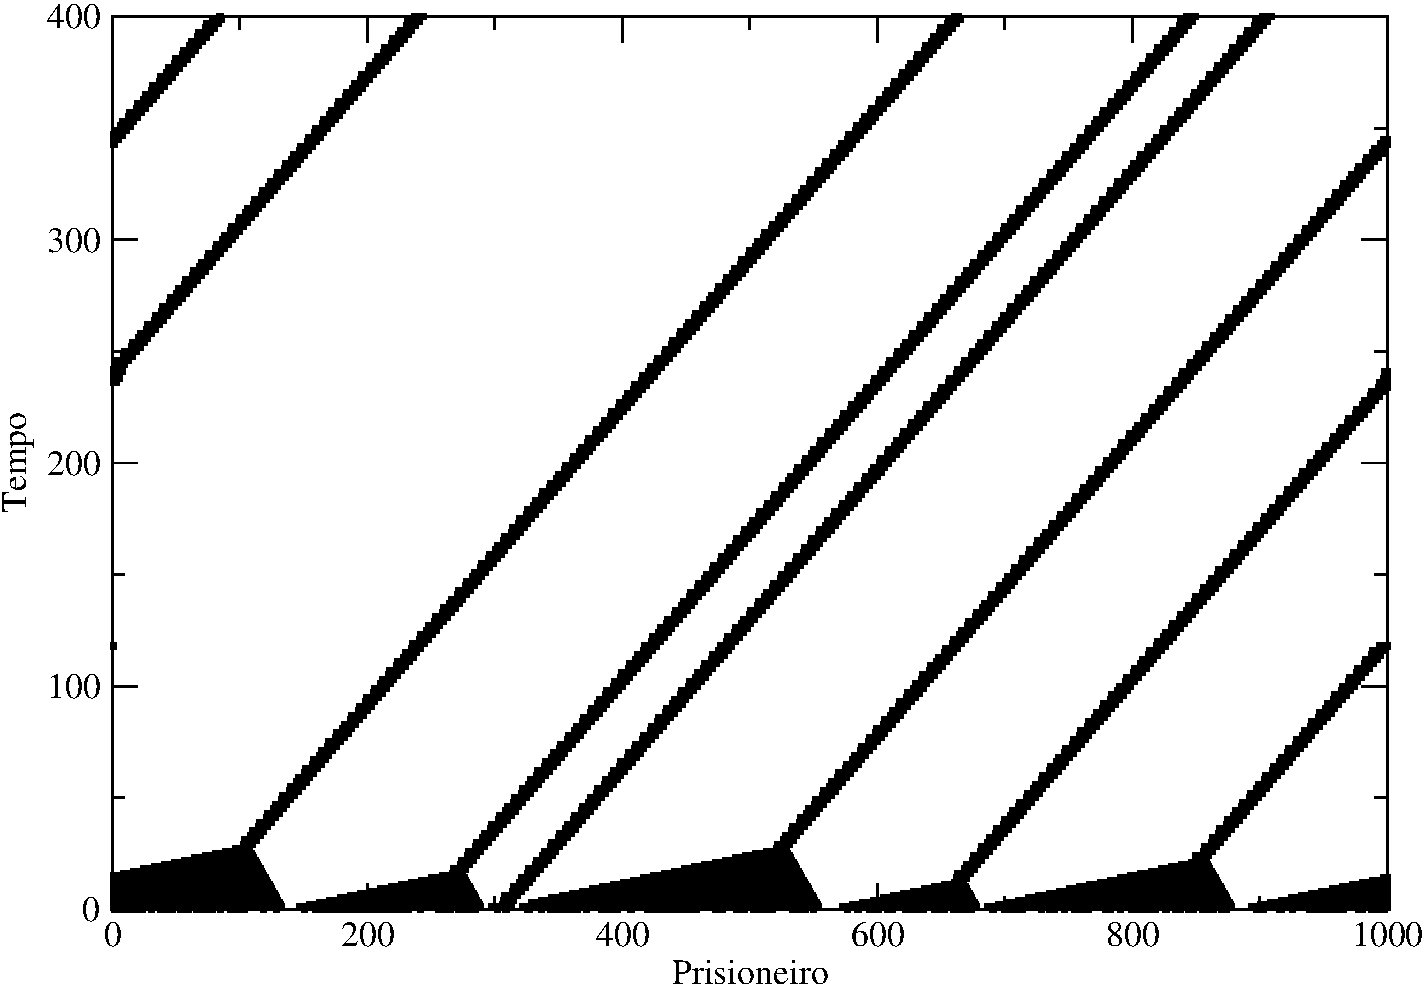
\includegraphics[width=0.4\textwidth]{z8_2.pdf}
\caption{Posição dos prisioneiros delatores em função do tempo para z = 8.}
\label{2b}
\end{figure}

\begin{figure}[!htb]
\centering
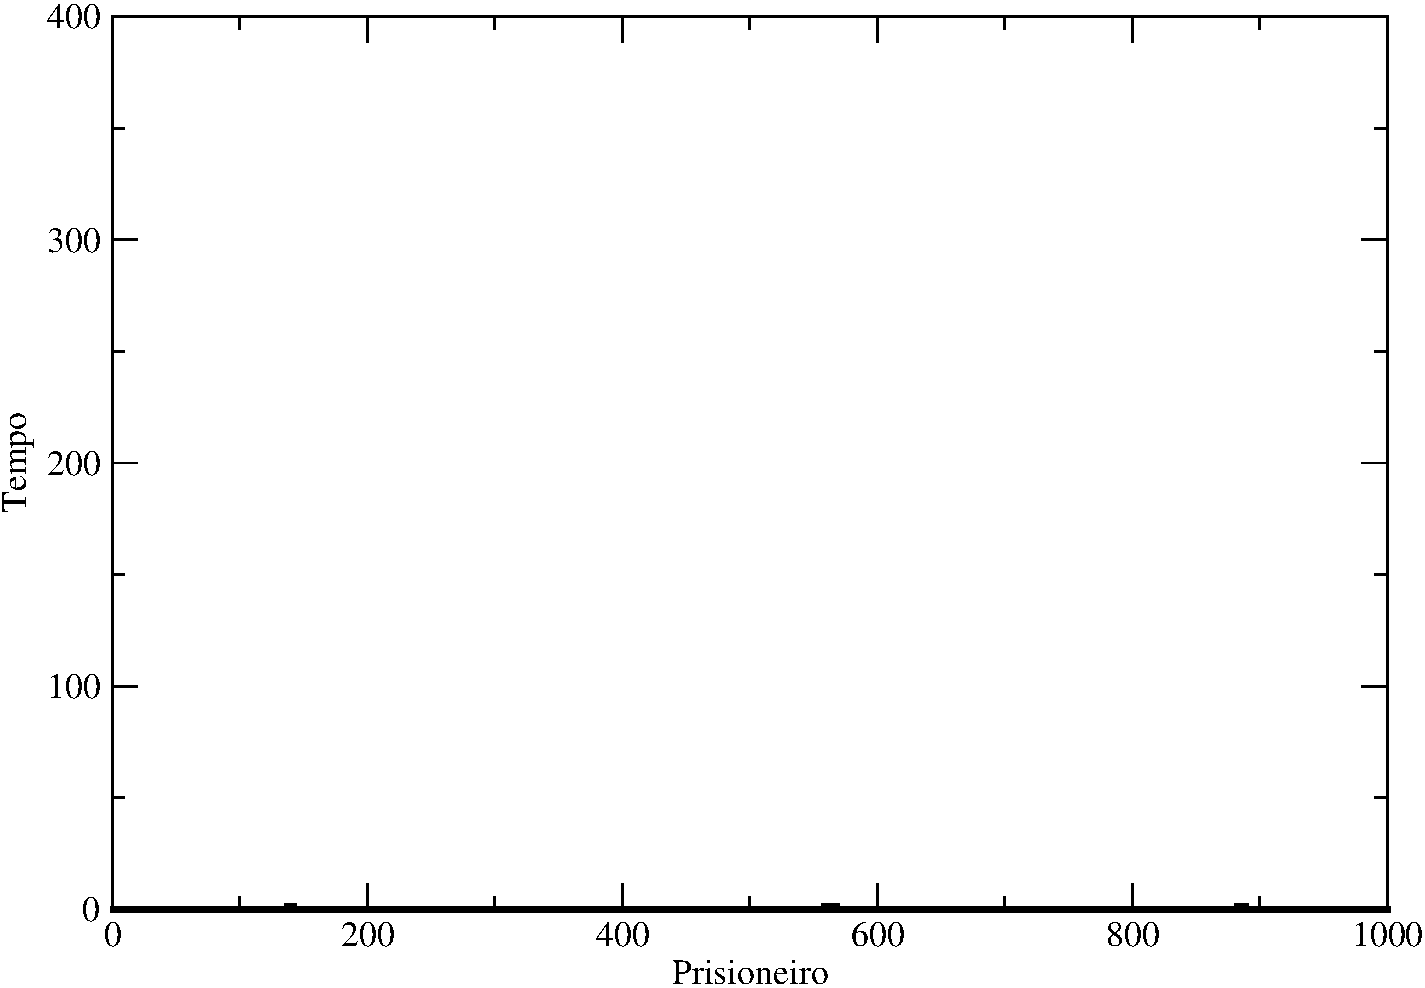
\includegraphics[width=0.4\textwidth]{z16.pdf}
\caption{Posição dos prisioneiros cooperando em função do tempo para z = 16.}
\label{3b}
\end{figure}

É interessante notar como os três casos são fundamentalmente diferentes. O caso z = 4 possui uma dinâmica que que atinge um estado estacionário; o caso z = 8 mostra uma dinâmica ue não parece atingir nenhum estado estacionário, pois os prisioneiros delatores parecem se propagar para a direita com velocidade constante; o caso z = 16 mostra uma dinâmica que rapidamente atinge um dos estados absorvetes.

\subsection*{c) }
O resultado da simulação está na Figura \ref{1c}. Foi escolhido as mesmas cores e símbolos do artigo original para que a comparação seja imediata.

\begin{figure}[!htb]
\centering
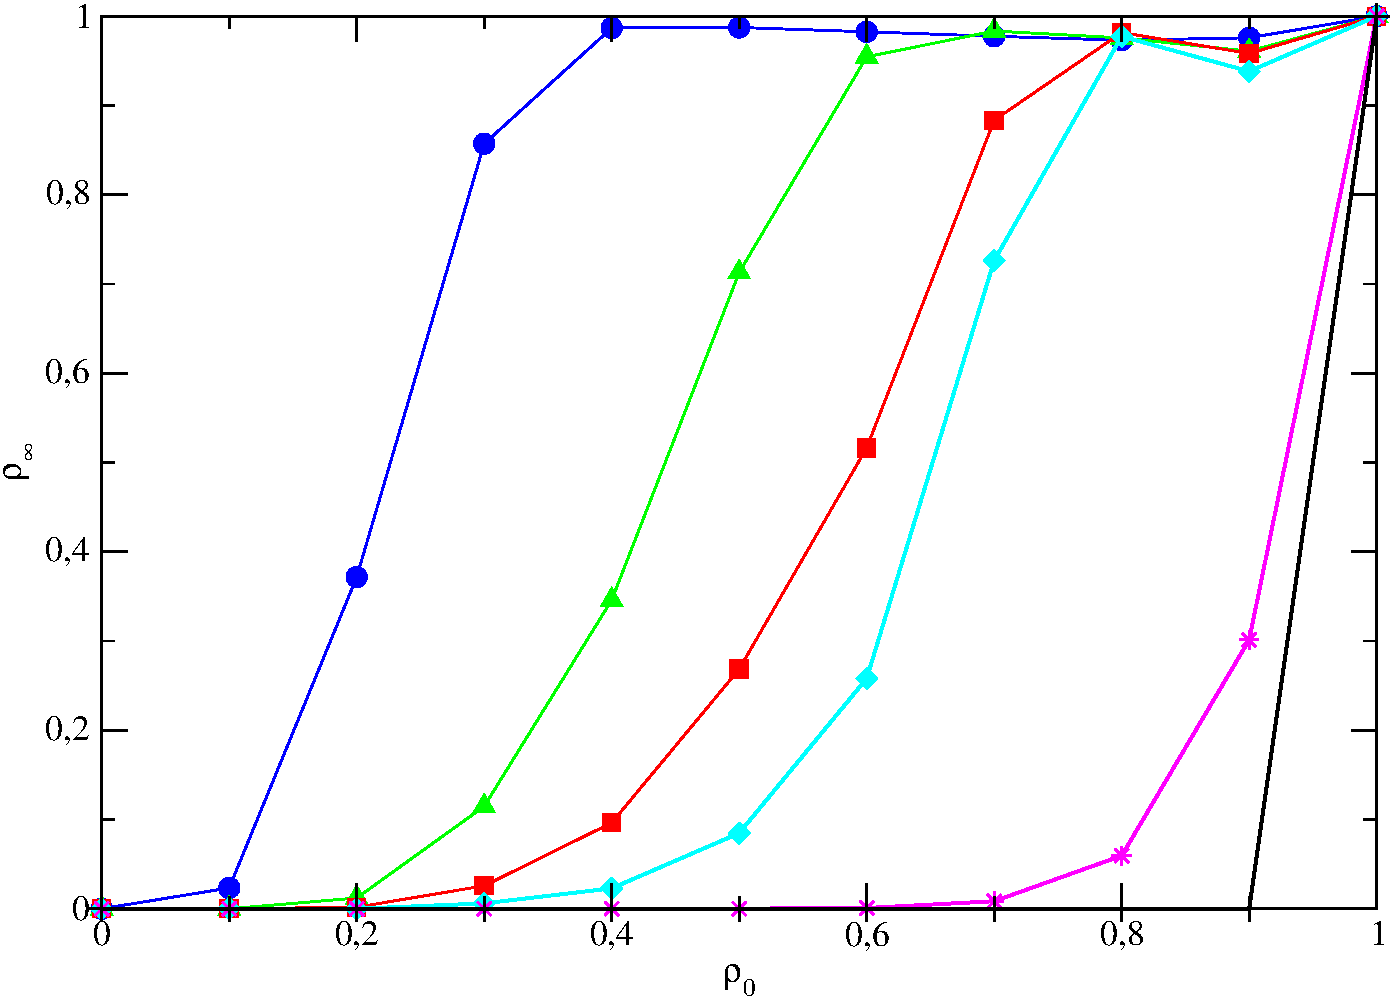
\includegraphics[width=0.4\textwidth]{infi.pdf}
\caption{$\rho_{\infty}$ em função de $\rho_{0}$ para z = 4. Linha preta: T = 2.0; Estrela roxa: T = 1.8; Diamante azul claro: T = 1.6; Quadrado vermelho: T = 1.4; Triangulo verde: T = 1.2; Círculo azul: T = 1.0. }
\label{1c}
\end{figure}


\section*{Exercício 2}
O programa está na pasta 2. Na Figura \ref{2aa} foi feito uma imagem de um cristal de tamanho n = 200 para termos ideia do tipo de estrutura formada.

\begin{figure}[!htb]
\centering
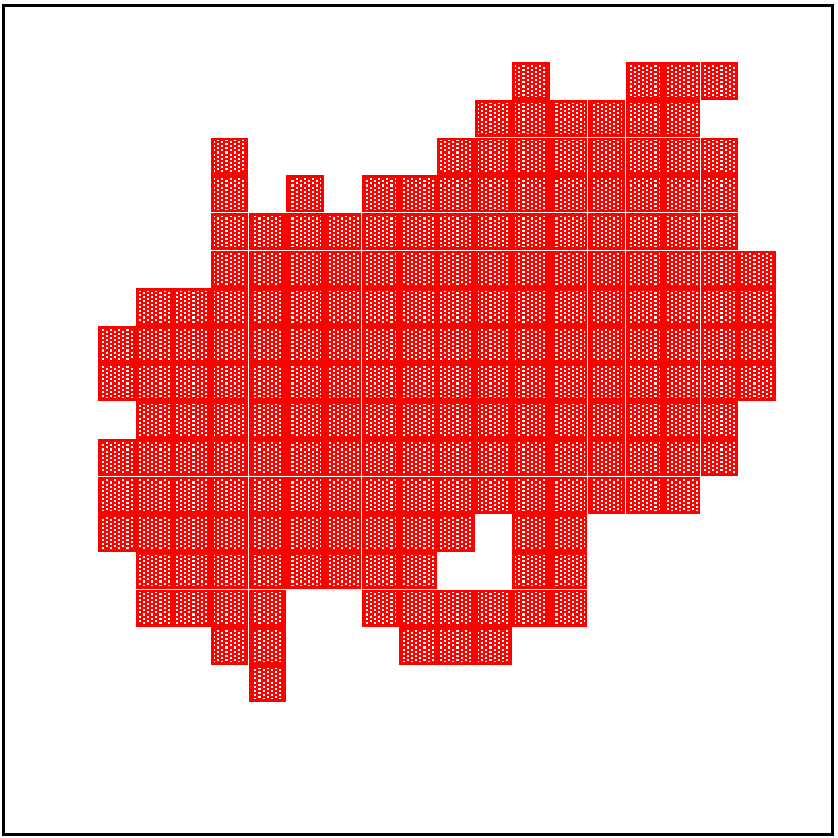
\includegraphics[width=0.4\textwidth]{cristal.pdf}
\caption{Exemplo de cristal de tamanho n = 200 formado.}
\label{2aa}
\end{figure}

Como os sítios com maior número de vizinhos são mais difíceis de serem removidos e as regras de criação/destruição são anisotrópicas é esperado que o cristal formado se aproxime de uma circunferência, evitando ao máximo regiões com pontas. Como pode ser visto na Figura \ref{2aa} isto é de fato o que se encontra.

\subsection*{a)}
Os gráficos foram feitos com $N_{0} = 7\times10^5$ para $s < 0.5$ visto que a estatística era ruim para $N_0 = 1000$. Para $s > 0.5$ foi usado $N_0 = 1\times10^5$. Plotar todos os 26 gráficos faria uma imagem excessivamente poluída, então foi escolhido plotar apenas alguns valores de s mais relevantes, o que pode ser visto na Figura \ref{2a}. Os gráficos P(n) restantes podem ser vistos na pasta Lista 14/2/Data. 

\begin{figure}[!htb]
\centering
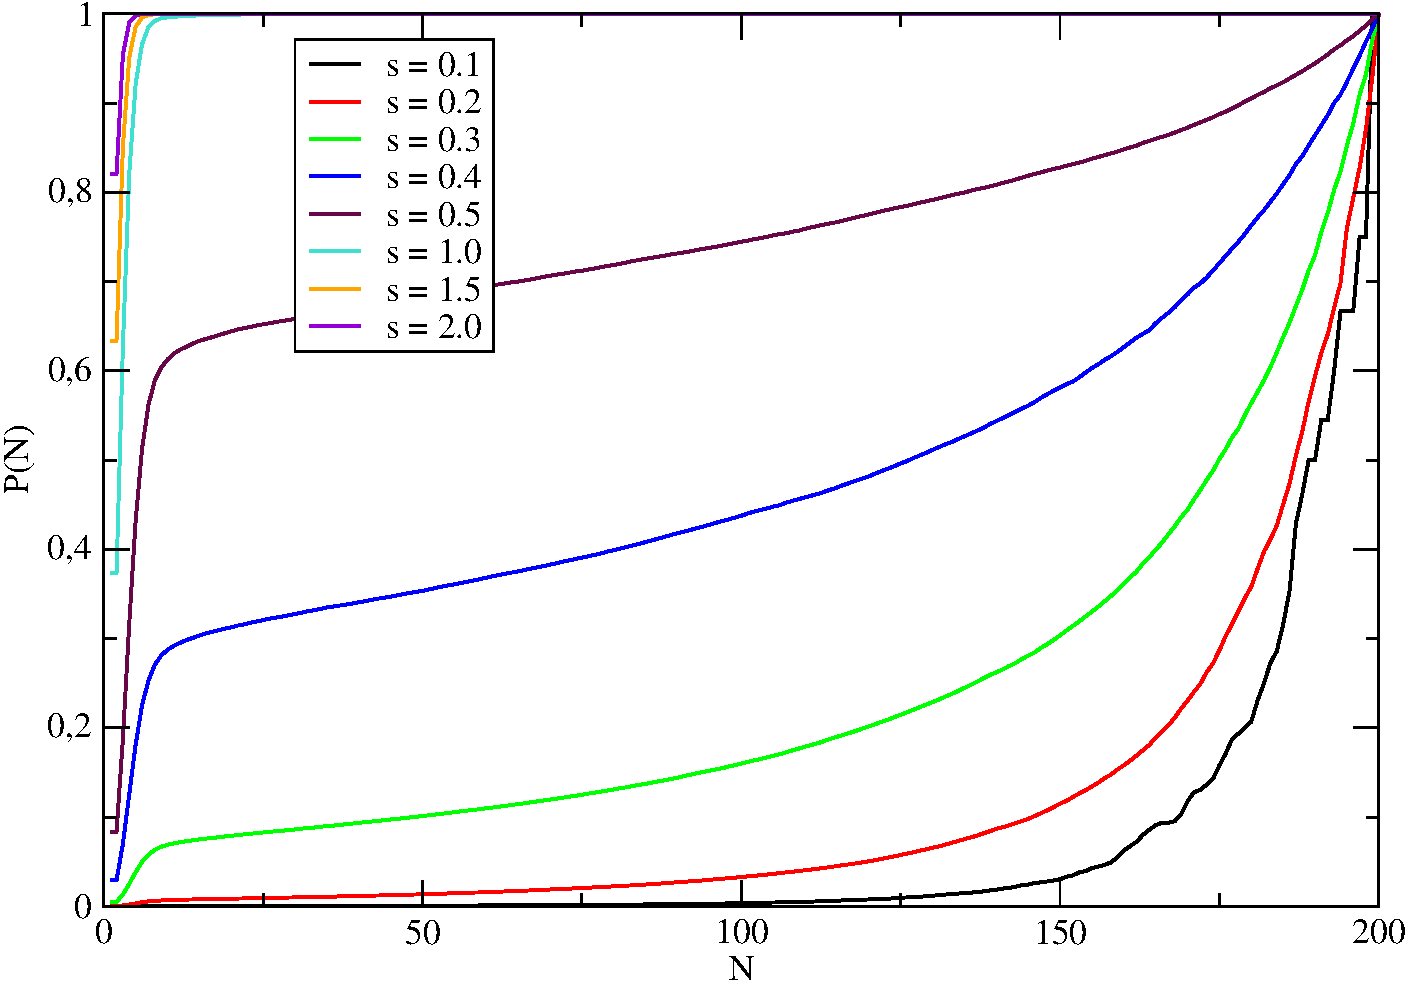
\includegraphics[width=0.4\textwidth]{pn.pdf}
\caption{P(n) em função de n para diferentes valores de saturação.}
\label{2a}
\end{figure}

\subsection*{b)}
Utilizando os gráficos de P(n) (como o que pode ser visto na Figura \ref{2a}) é possível obter para qual N temos $P(N) = 0.5$, ou seja, o N crítico tal que a probabilidade do cristal crescer para um tamanho macroscópico é igual à probabilidade de dissolução do agregado. O resultado pode ser visto na Figura \ref{2b}. É interessante notar como para s = 0.4 há um salto de aproximadamente uma ordem de grandeza.

\begin{figure}[!htb]
\centering
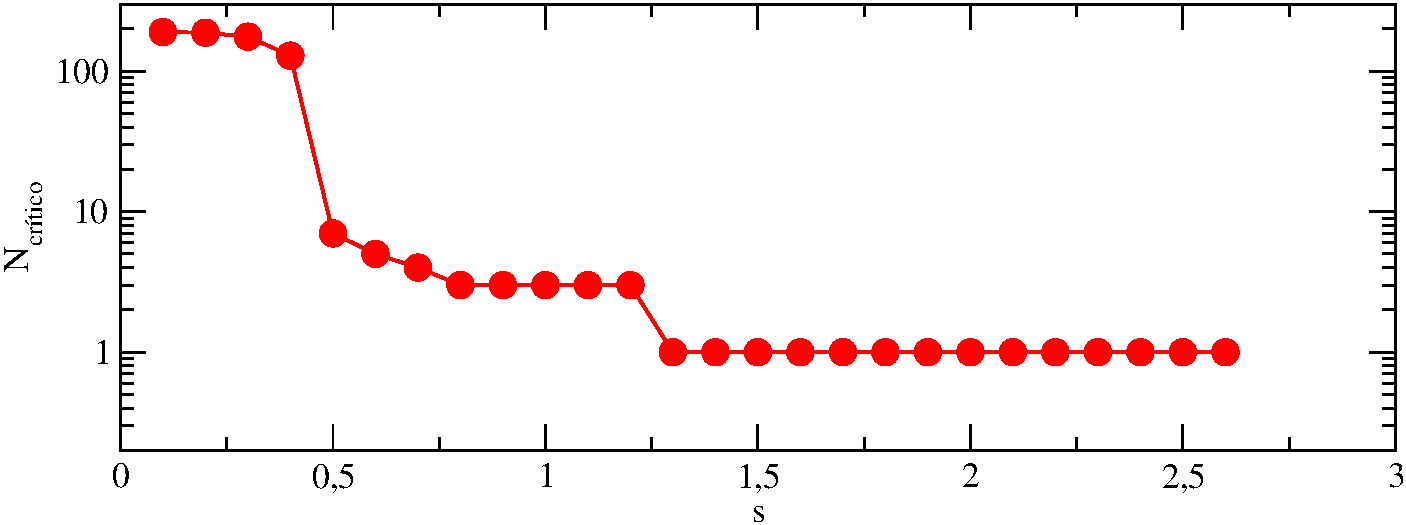
\includegraphics[width=0.4\textwidth]{nc.pdf}
\caption{Numero crítico $n_c$ em função da saturação.}
\label{2b}
\end{figure}


\subsection*{c)}
A probabilidade de um cristal atingir o tamanho $n_{max}$ pode ser obtida através da expressão $P_{2} = \frac{N(n_{max})}{N_0}$, onde $N_0$ é o número total de simulações realizadas. Na Figura \ref{2c} foi feito o gráfico de $P_2$ em função de s. O comportamento qualitativo é bem similar ao da referência [3].

\begin{figure}[!htb]
\centering
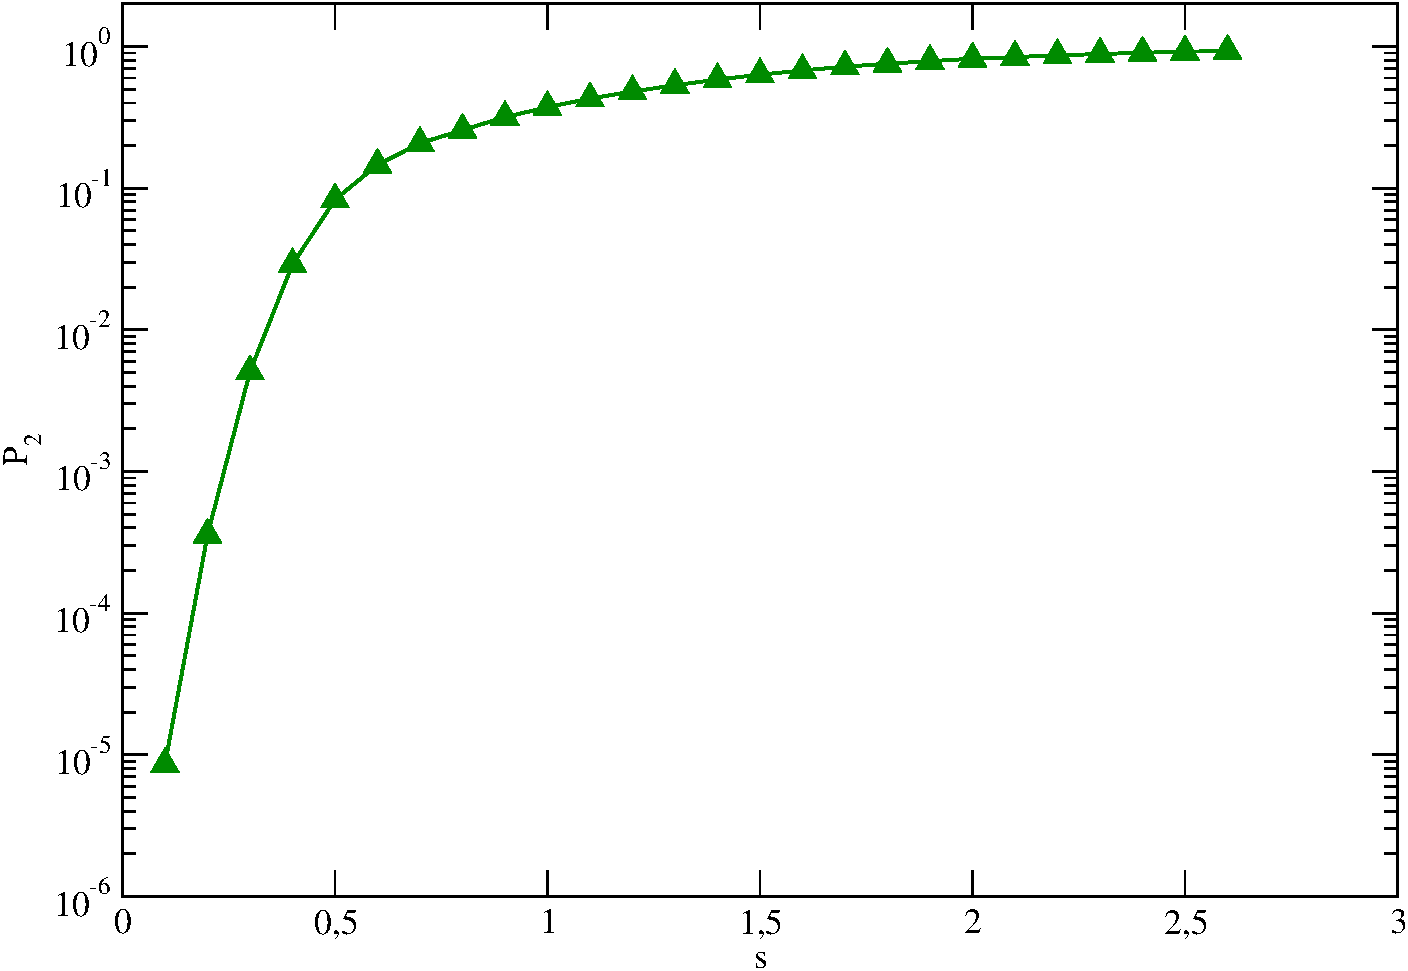
\includegraphics[width=0.4\textwidth]{p3.pdf}
\caption{Probabilidade $P_{2} = \frac{N(n_{max})}{N_0}$ em função da saturação s.}
\label{2c}
\end{figure}
\end{document}